
Section \ref{Sec:VolumeRegistrationSection} described techniques to register camera frames which have been projected to three dimensions. As mentioned, these frames may be registered with respect to the most common type of camera pose transform: y-axis rotation as well as camera movement. In addition, scale may be registered. For frames which have been projected differently or frames in which depth is computed relative to each frame, such as per frame depth computed in monocular view situations, this is an important transformation to register against. This is especially true since existing methods perform simple rigid movement camera pose registration. \\

This section integrates this method into a full 3D reconstruction algorithm. This algorithm may also be used to perform SLAM and it may still be applied to input data in which depth is not projected at correct scale between frames. The input for this method is RGB images, with a depth component. The data may be generated via an RGB-D camera or the depth may be computed implicitly across camera frames using frame calibration with a known stereo disparity method. Alternatively, stereo cameras may be set up initially in which depth data may be computed per frame using disparity methods directly for each frame. \\

Results for the FVR method are presented in section \ref{Sec:CamTransTrackExp}, \ref{Sec:CamRoteTrackExp}, \ref{Sec:FVRMotionExp} and \ref{Sec:FVRQual1Exp}. These show the FVR method is capable of accurate 3D reconstructions whilst being robust to noise. Details of how the Fourier Registration methods described in section \ref{FVRSectionA} are integrated to create the FVR algorithm. \\


\subsubsection{Pipeline}

\label{sec:FVRPipelineSect}

In figure \ref{fig:PIPELINENo1} a pipeline for the registration method is shown. This is a high level pipeline for the recovery of scale, y-axis rotation and translation. Much of the operations may be performed using GPU processing techniques. Signal Processing methods are so common, many hardware devices exist which are able to implement the techniques used in Fourier Volume Reconstruction. \\

Two volumes, $Volume_1$ and $Volume_2$ are both first put through a Hanning window function, these operations may be performed in parallel. Additionally this process multiples each voxel by a scalar which may be computed entirely based on location or a lookup volume pattern. So each Hanning window operation may also be performed on the GPU or using another parallel programming technique such as multi-threading. \\

Next, using the FFT the magnitude of the Discrete Fourier Transform is computed. The 3D FFT is a common operation which is implemented on most General Purpose Graphics Processing Units (GPGPUs). The 3D FFT operations on the GPGPUs produce the real and imaginary components of the frequency domain, but an additional GPU operation may be used to compute the magnitude values based on the real and imaginary values. Again this operation is easily extended to parallel processing platforms and both volumes may be transformed in parallel. \\

The Log(x) function is also a per voxel operation which may be computed on a parallel processing platform and both volumes may be transformed in parallel. The log-spherical transform may be computed for each volume at the same time and is inherently parallel. Additional memory requirements must also be met as both input and output volumes must be kept in memory simultaneously. \\

\begin{figure*}[!htb]
\centering
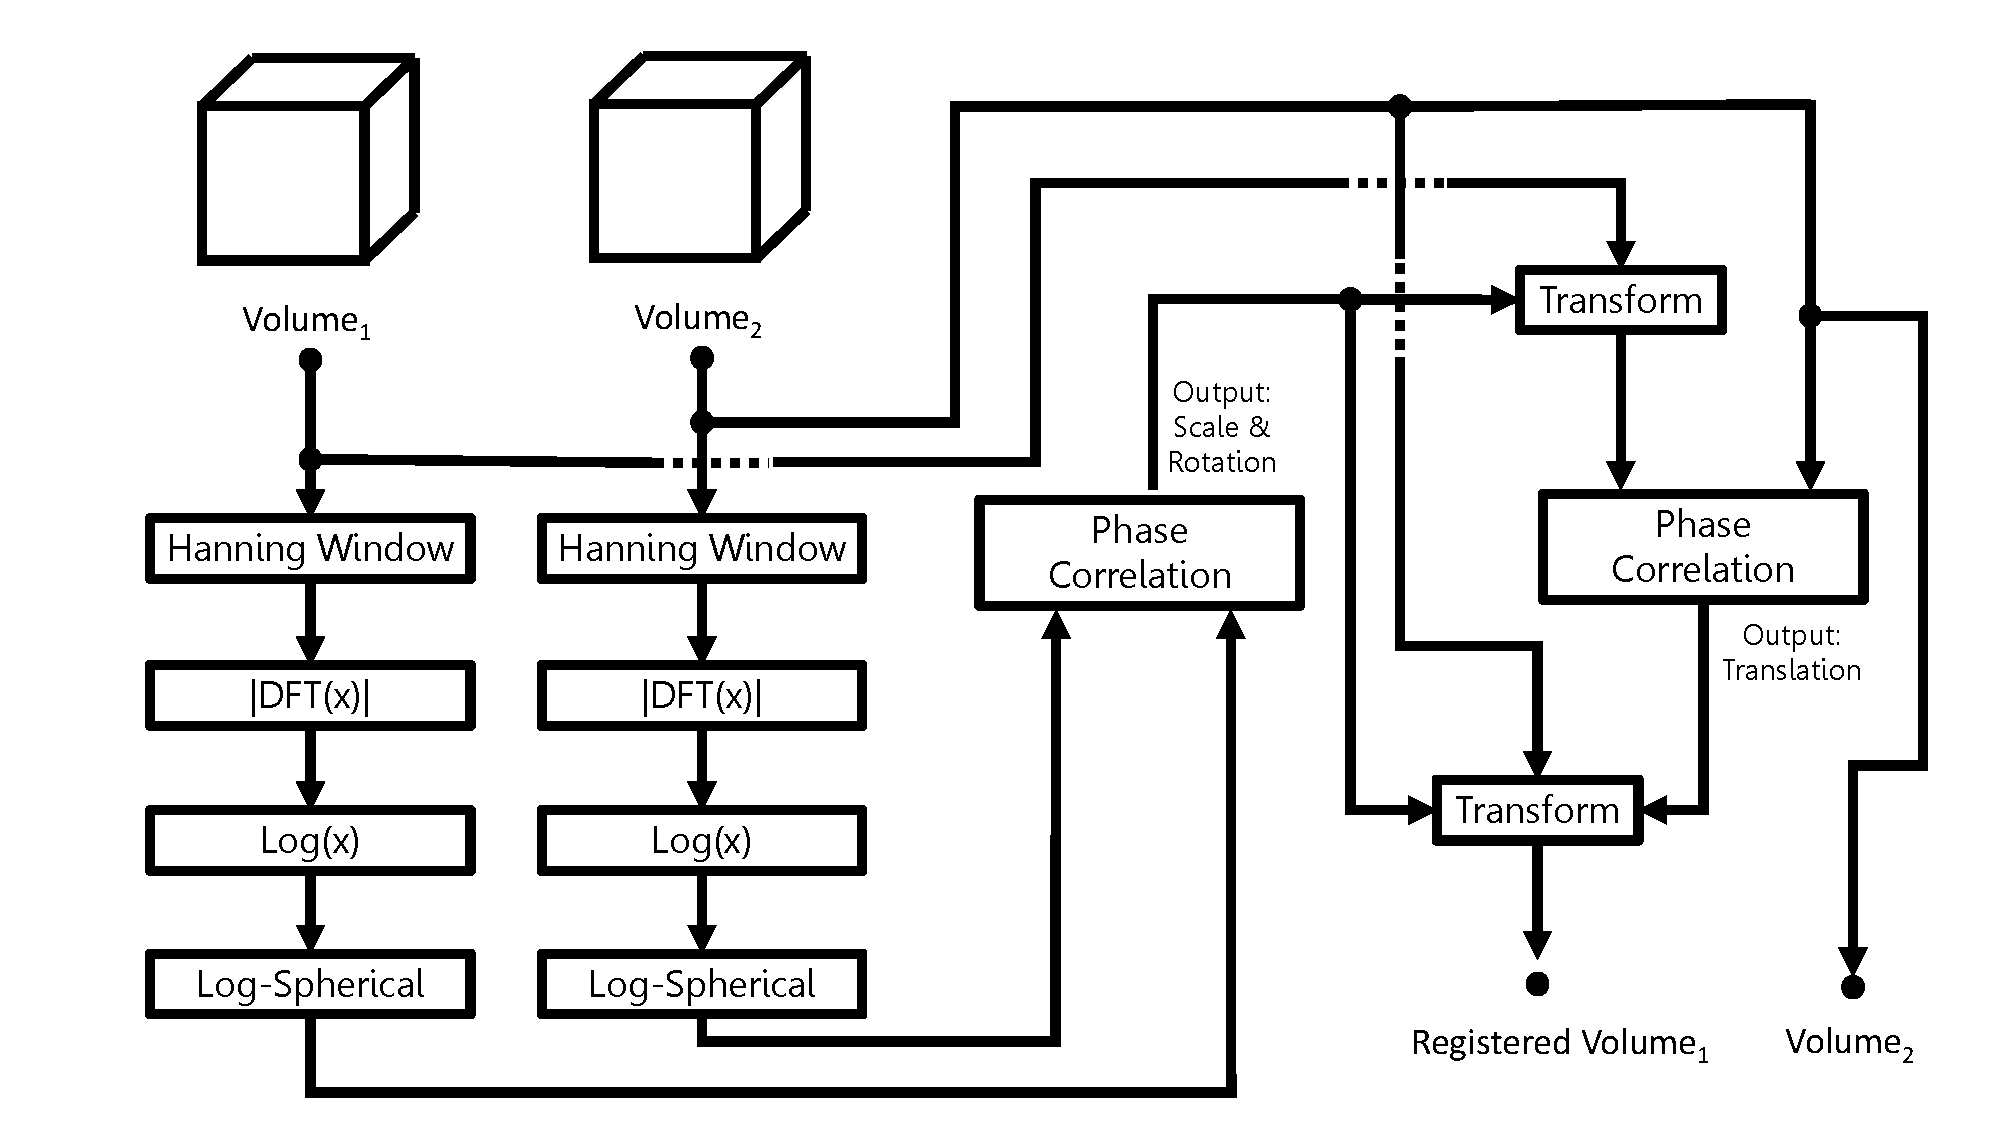
\includegraphics[width=6.0in]{images/ch2/pipeline2}
\caption{System Diagram for Registration Process}
\label{fig:PIPELINENo1}
\end{figure*}


The Phase Correlation operation is made up of multiple FFTs and their inverse, as well as computing the cross power spectrum for the volumes. All of these operations may be performed in GPGPUs. Searching for the output peak is an inherently sequential process. Parallel techniques such as reduction may be used but the performance gain is minimal. \\

Transforming the input volume is another process which may be performed using parallel techniques. The final phase correlation procedure is also parallel in nature apart from the peak value search on the phase correlation surface. \\



\subsubsection{Algorithm}

Using the Registration pipeline to compute the relationship between two frames, a SLAM and 3D reconstruction algorithm may be formulated. This algorithm can construct dense 3D reconstructions whilst simultaneously computing relative camera pose estimates. \\

 
The overall algorithm is presented in listings \ref{algorithm:PCSLAMNo1}. In the first line, the first frame is read as an RGB-D image into variable $f_1$. This RGB-D image is projected into a 3D point cloud representation using a projection function. The point cloud data for this first frame is then integrated into an automatically expanding occupancy grid representing the global 3D reconstruction output variable named $GlobalReconstruction$. \\

An accumulation matrix $M$ is used to formulate transforms for each frame read in. It is used by the algorithm to integrate frames directly into the output global reconstruction. Two variables $Camera_{location}$ and $Camera_{pose}$ are used to represent the camera location and pose information. The pose contains three vectors representing the camera space within the world space. A list of the camera locations and poses is referred to by the $Cameras$ variable. Each element in this list is a camera location and pose pair. \\

\begin{figure}
\begin{lstlisting}[language=c++,caption=Phase Correlation Based SLAM Algorithm,label=algorithm:PCSLAMNo1,mathescape,basicstyle=\ttfamily]
$f_1$ = ReadFrame();
$PointCloud$ = project($f_1$);
$GlobalReconstruction$.integrate($PointCloud$)
$M$ = IdentityMatrix();
$Camera_{location}$ = $[0, 0, 0]^T$;
$Camera_{pose}$ = $[[1, 0, 0]^T,[0, 1, 0]^T,[0, 0, 1]^T]$;
$Cameras$ = $\left[\left[Camera_{location}, Camera_{pose}\right] \right]$;
while(more frames){
	$f_2$ = ReadFrame();
	$points_1$ = project($f_2$);
	$points_2$ = project($f_1$);
	$V_1$ = Voxelize($points_1$);
	$V_2$ = Voxelize($points_2$);
	$(\theta, \varphi, t_x, t_y, t_z) = VR_{\theta \varphi t_x t_y t_z}(V_1, V_2)$;
	$Temp = $TransformMat($(\theta, \varphi, t_x, t_y, t_z)$);
	$M = M \times Temp$;
	$points_1$ = Transform($points_1$, $M$);
	$GlobalReconstruction$.integrate($points_1$);
	$Camera_{location}$ = $Temp^{-1} \times Camera_{location}$;
	$Camera_{pose}$ = $Temp^{-1} \times (Camera_{pose} + Camera_{location})$;
	$Camera_{pose}$ = $\frac{Camera_{pose} - Camera_{location}}{Camera_{pose} - Camera_{location}}$;
	$Cameras.add(\left[Camera_{location}, Camera_{pose}\right])$;
	$f_1$ = $f_2$;
}
\end{lstlisting}
\end{figure}

The algorithm iterates over each frame pair which must be registered and integrated. Each iteration begins by reading in a new frame. This is pointed to by variable $f_2$. Next, both $f_1$ and $f_2$ are projected into point clouds named $points_1$ and $points_2$ respectively. The Fourier Volume Reconstruction method requires the frames be integrated into 3D volumes, so the Voxelize function is used to integrate the points and color information into the volumes. \\

The FVR method works with either integrated greyscale information based on the RGB data, or with raw occupancy values. The use of RGB data may have slight performance implications. Many computer vision algorithms prefer to work in greyscale, especially feature matching methods. This is often due to a combination of complexity and performance reasons. Whilst colour information does improve accuracy, it is considered to be minimal relative to savings in computational complexity. \\

Integrating the colour information for use in the FVR method does not incur any performance penalty. The only shortcoming of using the extra colour information to increase accuracy is the loss of the ability to work in total darkness using RGB-D sensors. \\

As mentioned in the literature, the Kinect Fusion technique only makes use of depth information which is obtained via an active camera (the Kinect). In this way is can effectively work in the dark. If the FVR method uses colour information integrated directly, and the colour components do not pick up any light. The method will fail. This can be easily detected and because FVR also works by simply registering occupancy volumes, it can switch over to this upon detecting that no colour (visible light) information is available. \\

Once the volumes are reconstructed, the rotation, scale and translation factors may be computed using the pipeline discussed in section \ref{sec:FVRPipelineSect}. A transformation matrix, $Temp$ may then be created from these values. Such a matrix was presented in section \ref{FVRSectionA}. $M$ is then updated to itself times the computed transformation matrix $Temp$. In this way, $M$ can be used to accumulate previous registrations. \\

The $points_1$ point cloud is then transformed by the newly computed $M$. The point cloud can then be integrated into the global reconstruction. Next, the camera location and pose list must be updated. The camera location is adjusted by the inverse of the newly computed $Temp$ matrix. As mentioned, the camera transforms will be related to the registration transforms inversely. \\

The camera pose is also updated, by adjusting the axes relative to the camera location using the $Temp$ matrix. The camera pose vectors are then normalized and added into the list of camera locations and poses. Finally, $f_1$ is set to $f_2$. In this way the algorithm can repeat with $f_1$ as the previously input frame. \\  



\subsubsection{Integration}

The integration procedure used with this technique is the common global voxel integration method. An automatically expanding volume is used to store the global 3D reconstruction. Given the algorithm described above, the output global reconstructed volume must take in point cloud data, and integrate it into the volume. \\

The algorithm proposed does not make use of loop closure. Many recent techniques also forgo the use of such procedures, especially if they integrate globally. The FVR method can also easily be adjusted by changing the last line of the algorithm. Rather than simply setting $f_1$ to $f_2$, $f_1$ may be set to the volume extracted by sampling the global reconstruction into a volume based on the most recent camera location and pose computed. This way, loops may be detected by registering upcoming frames globally. \\


\subsubsection{Limitations}

The FVR method is capable of registering 3D pose data and in turn can generate accurate, high quality 3D reconstructions. However, it is limited to a single axis of rotation (the y-axis). The FVR method was tested, and remains robust to up to 10 degrees of rotation along the other axes, however this method is still not able to register 3 degrees of rotation on its own. In order to move past this limitation whilst retaining the robustness and accuracy of the technique, a novel extension is proposed in section \ref{FullRecovery3DSection}. Both the FVR method and this extension are tested empirically in section \ref{ch:Experiments} and results show they outperform the current standard in 3D pose estimation and 3D reconstruction. \\